\newcommand{\dplothere}[2]{%
\begin{figure}[htb]
\centering
\begin{subfigure}{\linewidth}
\centering
    \includegraphics[height=0.48\textheight]{plots/#1-1}
\end{subfigure}
\par\bigskip % force a bit of vertical whitespace
\begin{subfigure}{\linewidth}
\centering
    \includegraphics[height=0.48\textheight]{plots/#1-2}
\end{subfigure}
\caption{#2}
\label{fig:#1}%
\end{figure}
}
\section{Ερώτημα Γ}
Υλοποιήθηκαν οι εξής εκδοχές του αλγορίθμου \emph{Block LMS}:
\begin{enumerate}[a)]
\item \label{item:simple}\texttt{lms/blocklms\_simple.m}: Με δύο εμφωλευμένους βρόχους.
\item \label{item:array}\texttt{lms/blocklms\_array.m}: Με ένα βρόχο και πράξεις πινάκων.
\item \label{item:fft}\texttt{lms/blocklms\_fft.m}: Με προσαρμογή στο πεδίο της συχνότητας κάνοντας χρήση του FFT.
\item \label{item:ufft}\texttt{lms/blocklms\_unconstrained\_fft.m}: Με μη περιορισμένη (unconstrained) προσαρμογή στο πεδίο της συχνότητας.
\end{enumerate}

Η πιο συμφέρουσα υπολογιστικά υλοποίηση είναι αυτή με τη
\hyperref[item:ufft]{μη περιορισμένη προσαρμογή στο πεδίο της συχνότητας}.
Το σχετικό διάγραμμα φαίνεται στο \imageref{performance}.
Στα αρχεία \texttt{profiler\_results/file*.html} φαίνεται αναλυτικά ο χρόνος εκτέλεσης για κάθε συνάρτηση για \mintinline{MATLAB}!n = 45000!.
\dplothere{performance}{Ταχύτητα εκτέλεσης των 4 αλγορίθμων LMS}

Τέλος, οι καμπύλες εκμάθησης για τους αλγορίθμους φαίνονται στο \imageref{learning-curve}.
Παρατηρούμε ότι για τους 3 πρώτους αλγορίθμους οι καμπύλες εκμάθησης είναι ίδιες αφού οι αλγόριθμοι είναι ισοδύναμοι.
\begin{figure}
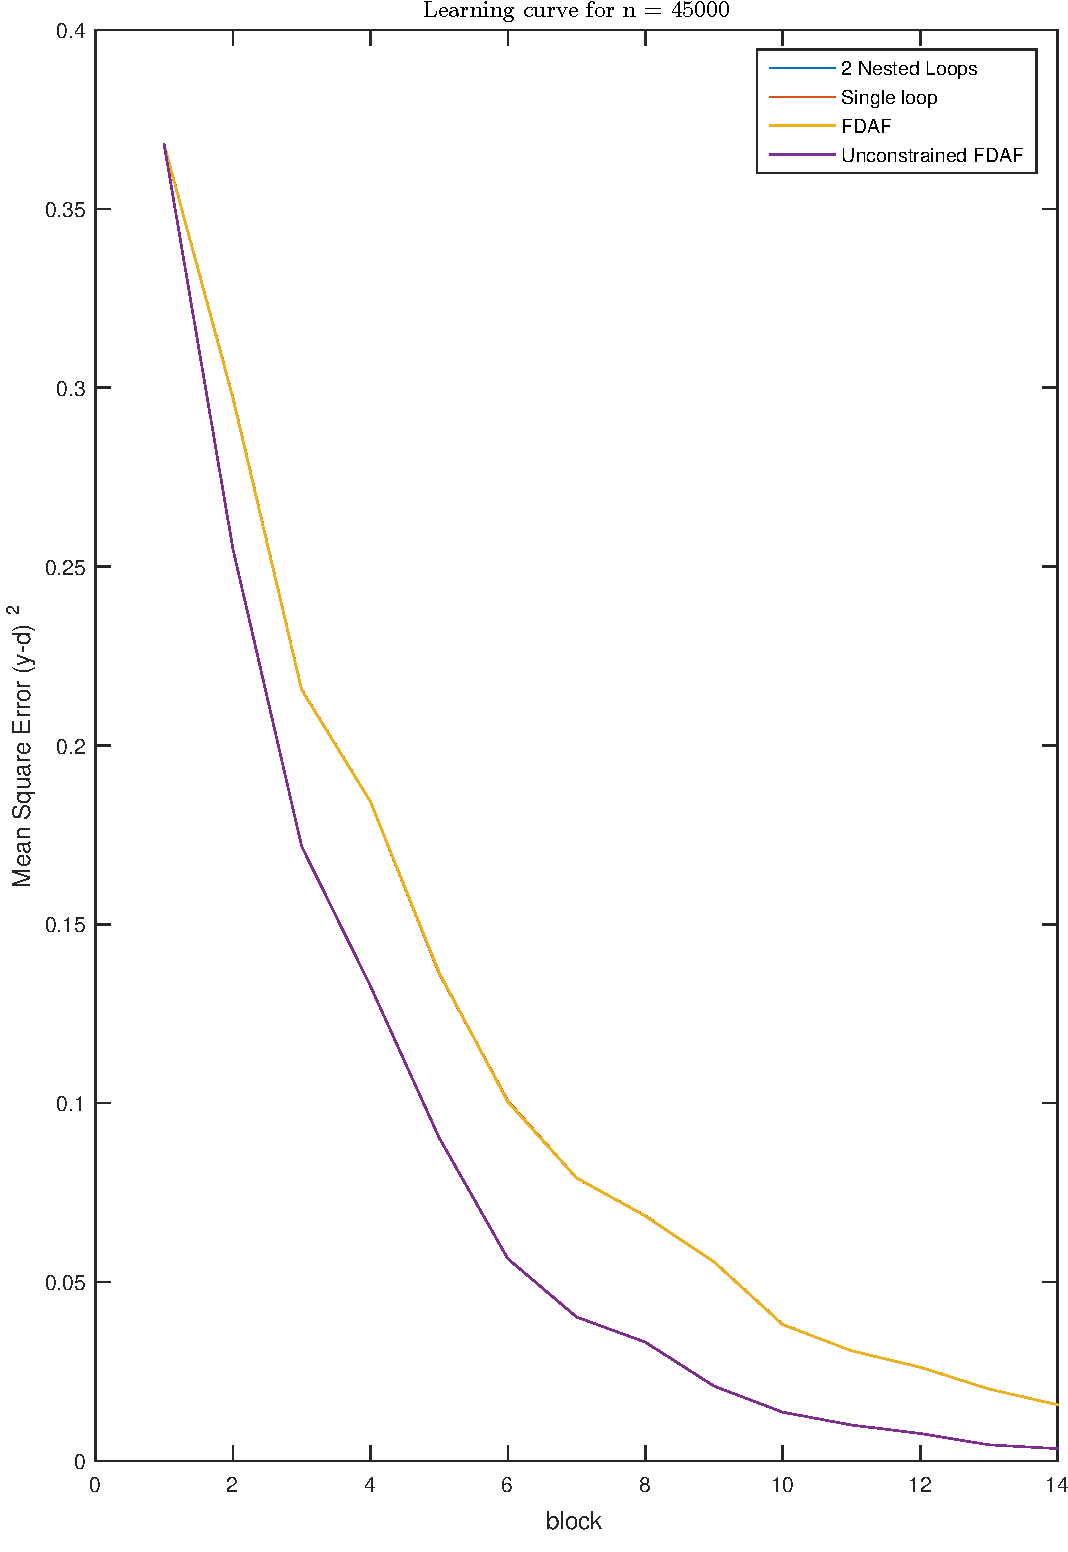
\includegraphics[width=\linewidth]{plots/learning-curve}
\caption{Καμπύλες εκμάθησης των 4 αλγορίθμων LMS}
\label{fig:learning-curve}
\end{figure}
